\documentclass[11pt]{article}

\usepackage{caption}
\usepackage{graphicx}
\usepackage{booktabs}
\usepackage[margin=0.88in]{geometry}
\usepackage{amsmath}
\usepackage{titlesec}
\usepackage{enumerate}
\usepackage{bm}
\usepackage{subfig}
\usepackage{wrapfig}

\setlength{\parindent}{0pt}

\begin{document}
	\begin{titlepage}
	\begin{flushleft}
	Imperial College London \\
	Department of Aeronautics \\
	Third Year HPC Coursework Report 2020 \\
	\end{flushleft}
	\vspace*{\fill}	
	\begin{center}
		\textsc{\Huge High Performance Computing Coursework} \\
		\vspace{11pt}
		\textit{\small Done by:} \\
		\textsc{\Large Chai Jun, Sean} \\
		\textsc{CID: 01327446} \\ 
		\vspace*{\fill}
	\end{center}
		
	\end{titlepage}
	
	\section{Result of running Lid Driven Cavity Solver}
	\subsection{Velocity Plots}
	\begin{figure}[htp]
            \centering
            \subfloat[Horizontal velocity $u$ against $y$ along $x=0.5$]{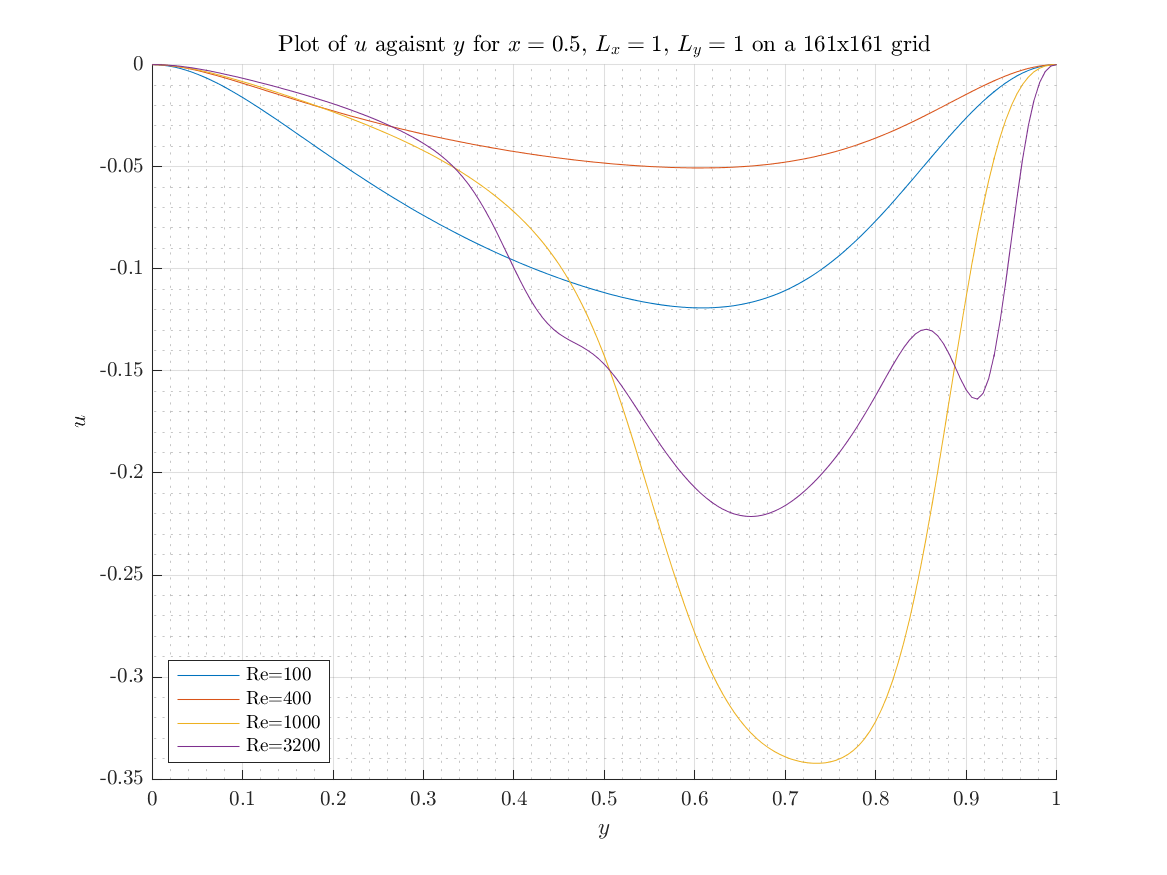
\includegraphics[width=0.48\textwidth]{../Images/u_vs_y.png}}
            \hfill
            \subfloat[Vertical velocity $v$ against $x$ along $y=0.5$]{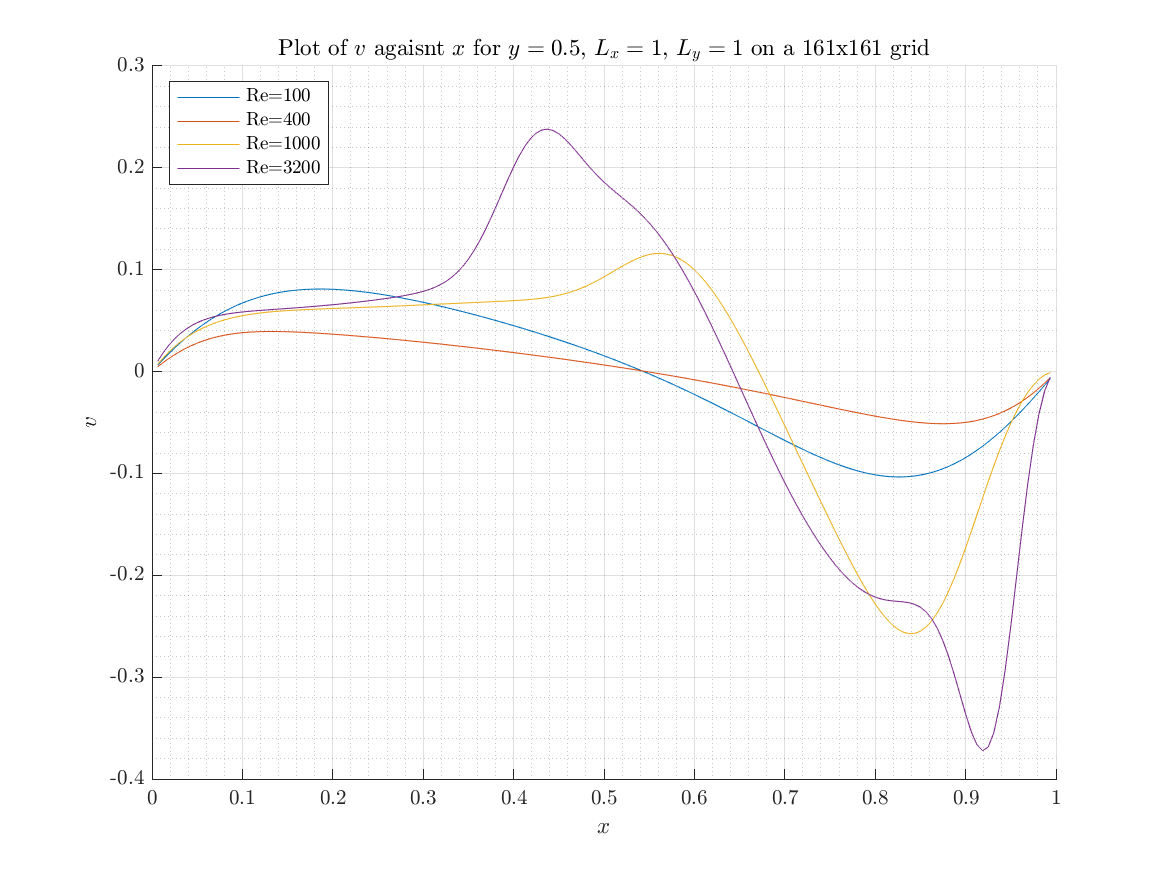
\includegraphics[width=0.48\textwidth]{../Images/v_vs_x.png}}
            \caption{Plot of velocities of the steady state solution for Reynolds numbers of 100, 400, 1000 and 3200 using a $161 \times 161$ grid and $L_x = L_y = 1$.}
            \label{fig:velocities}
        \end{figure}
	
	\subsection{Vorticity and Streamfunction}
	\begin{figure}[htp]
            \centering
            \subfloat[Vorticity contour plot]{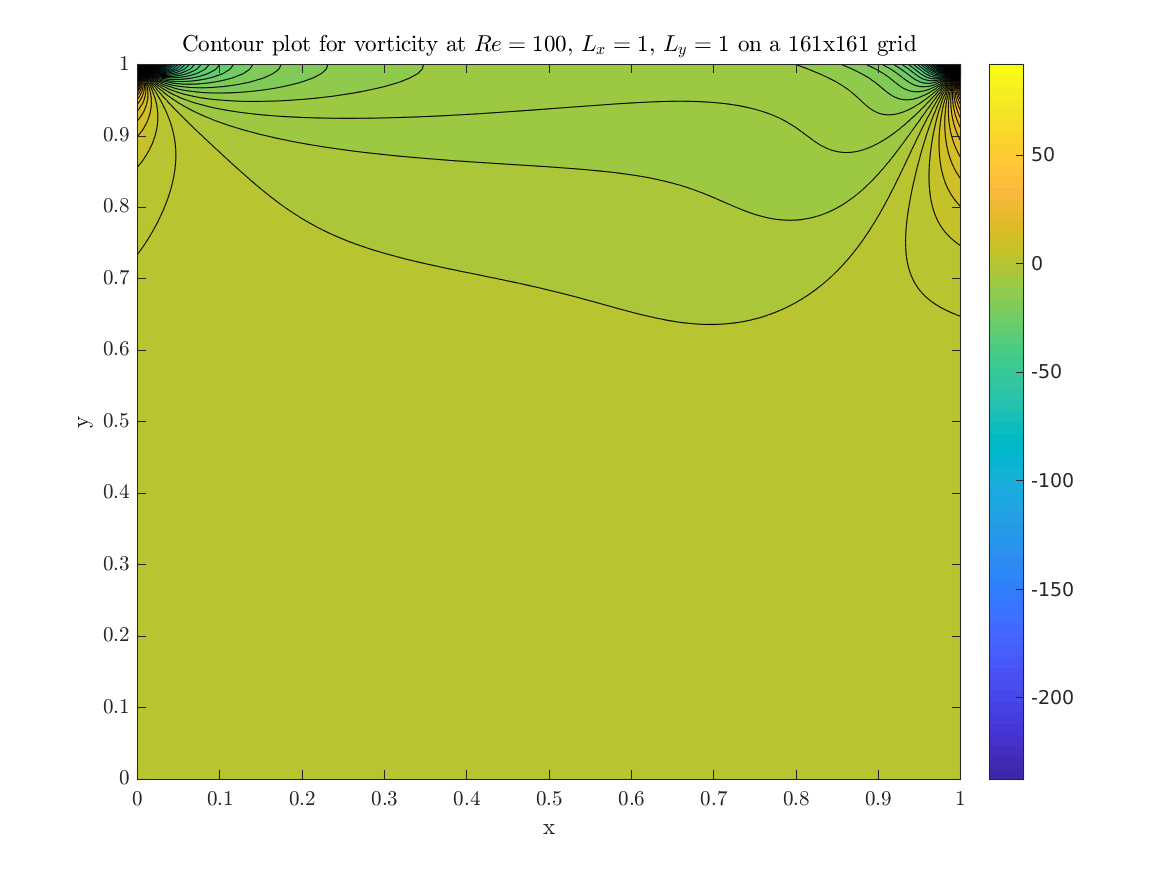
\includegraphics[width=0.48\textwidth]{../Images/w_100.png}}
            \hfill
            \subfloat[Streamfunction contour plot]{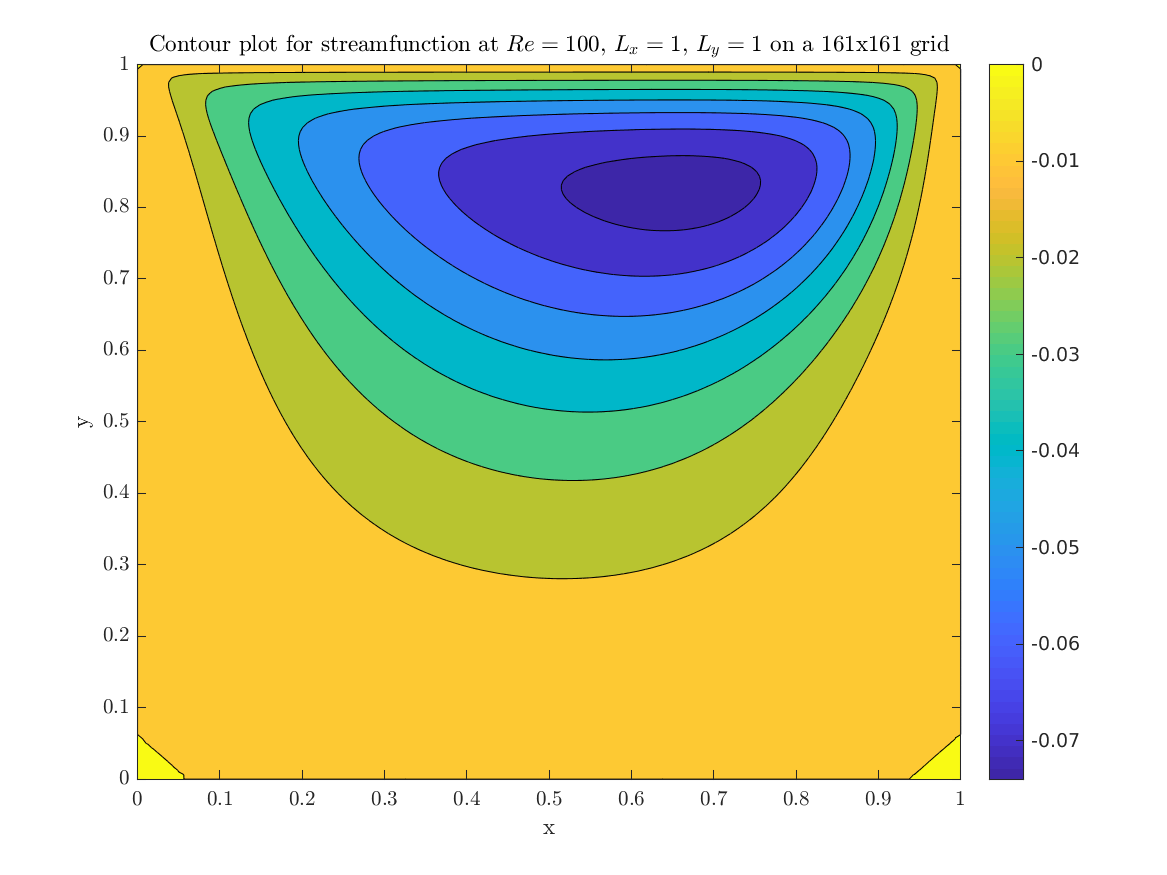
\includegraphics[width=0.48\textwidth]{../Images/s_100.png}}
            \caption{Contour plots of vorticity and streamfunction at $Re=100$ on a $161 \times 161$ grid and $L_x = L_y = 1$.}
            \label{fig:contours}
        \end{figure}			
	\newpage
	
	\subsection{Minimum Streamfunction}
	\begin{table}[htb]
    	\centering
    	\begin{tabular}{ c | c c c c }
    	\toprule
    	Reynolds Number & 100 & 400 & 1000 & 3200 \\
    	\midrule
		x-coordinate & 0.6562 & 0.8250 & 0.6875 & 0.6500 \\
		y-coordinate & 0.8250 & 0.8812 & 0.6875 & 0.6188  \\
        \bottomrule
        \end{tabular}
        \vspace{0.5em}
        \label{tab:stress}
    	\caption{Table of x-y coordinates of the streamfunction minimum at the different Reynolds numbers for a $161 \times 161$ grid and $L_x = L_y = 1$.}	
	\end{table}

	
	\subsection{Streamfunction Plots for Varying $L_x$ and $L_y$}
	\begin{figure}[htp]
            \centering
            \subfloat[$L_x=1$, $L_y=2$]{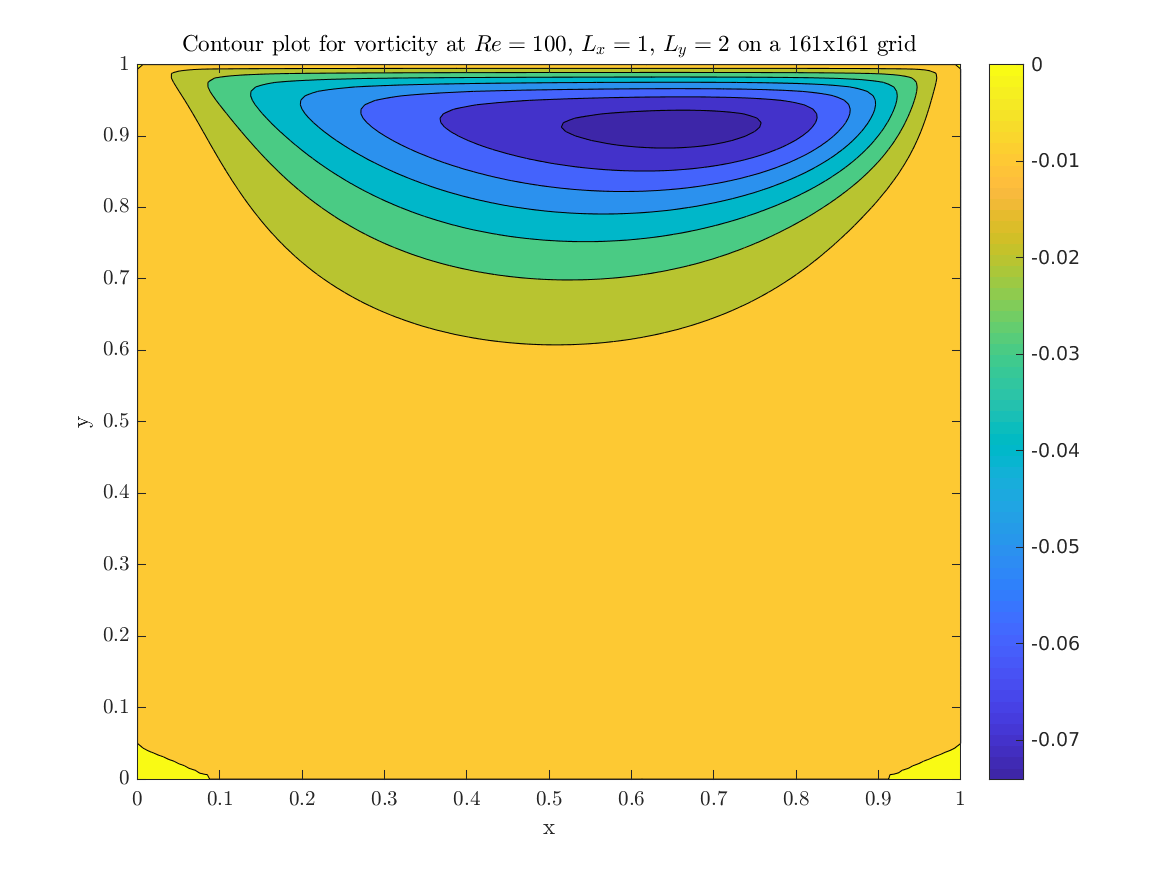
\includegraphics[width=0.45\textwidth]{../Images/lx1ly2.png}}
            \hfill
            \subfloat[$L_x=2$, $L_y=1$]{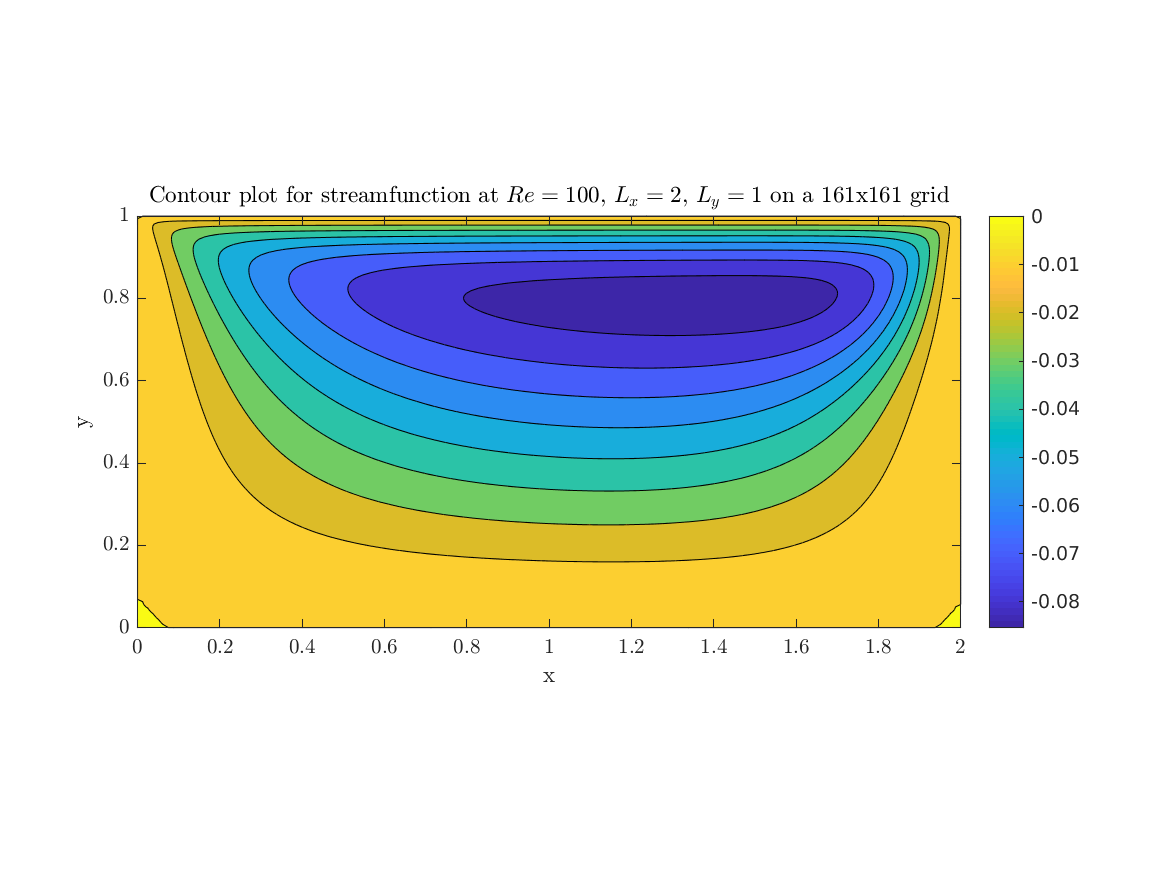
\includegraphics[width=0.55\textwidth]{../Images/lx2ly1.png}}
            \caption{Contour plots of  streamfunction at $Re=100$ on a $161 \times 161$ grid.}
            \label{fig:contours}
        \end{figure}	
	
	
%	\begin{figure}[htb]
%		\centering
%		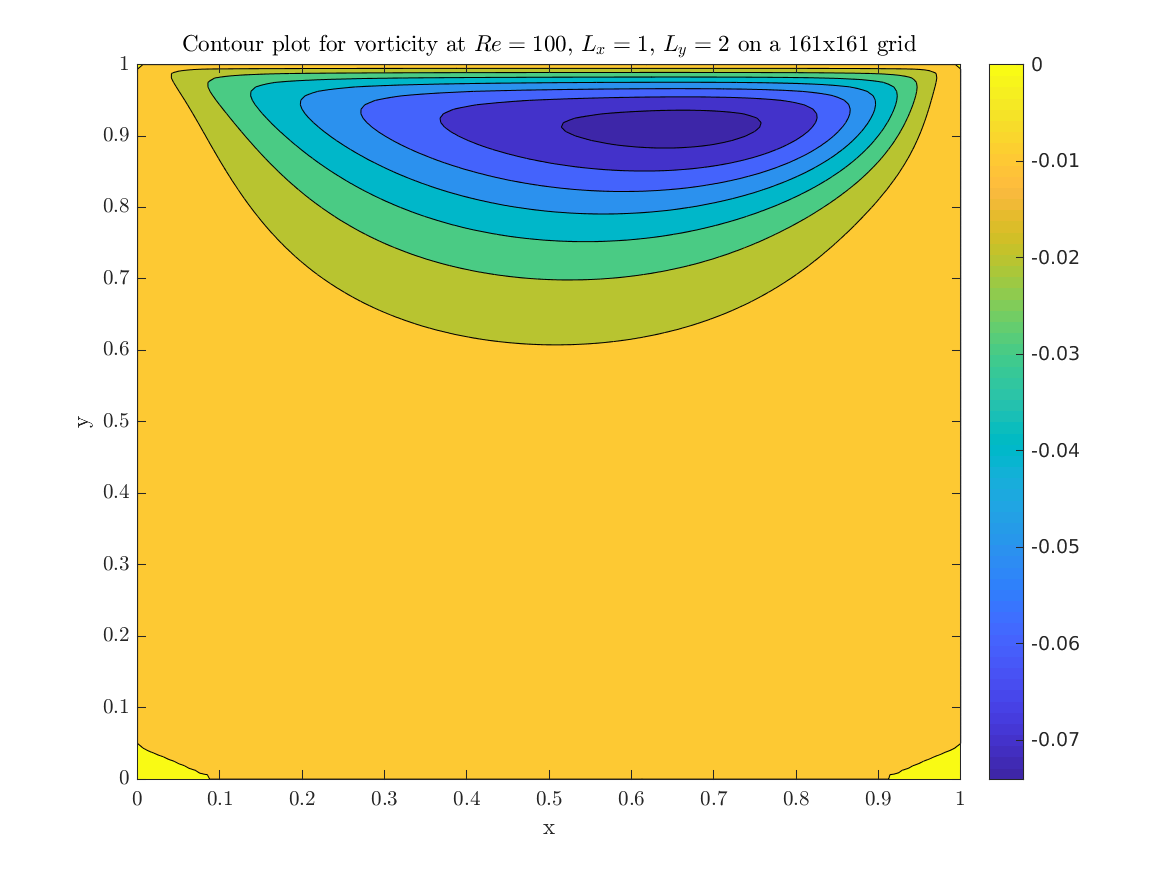
\includegraphics[width=0.45\linewidth]{../Images/lx1ly2.png}
%		\captionof{figure}{Contour plot of streamfunction at $Re=100$ on a $161 \times 161$ grid and $L_x = 1, \, L_y = 2$.}
%		\label{fig:s_100}
%	\end{figure}
%	
%	\begin{figure}[htb]
%		\centering
%		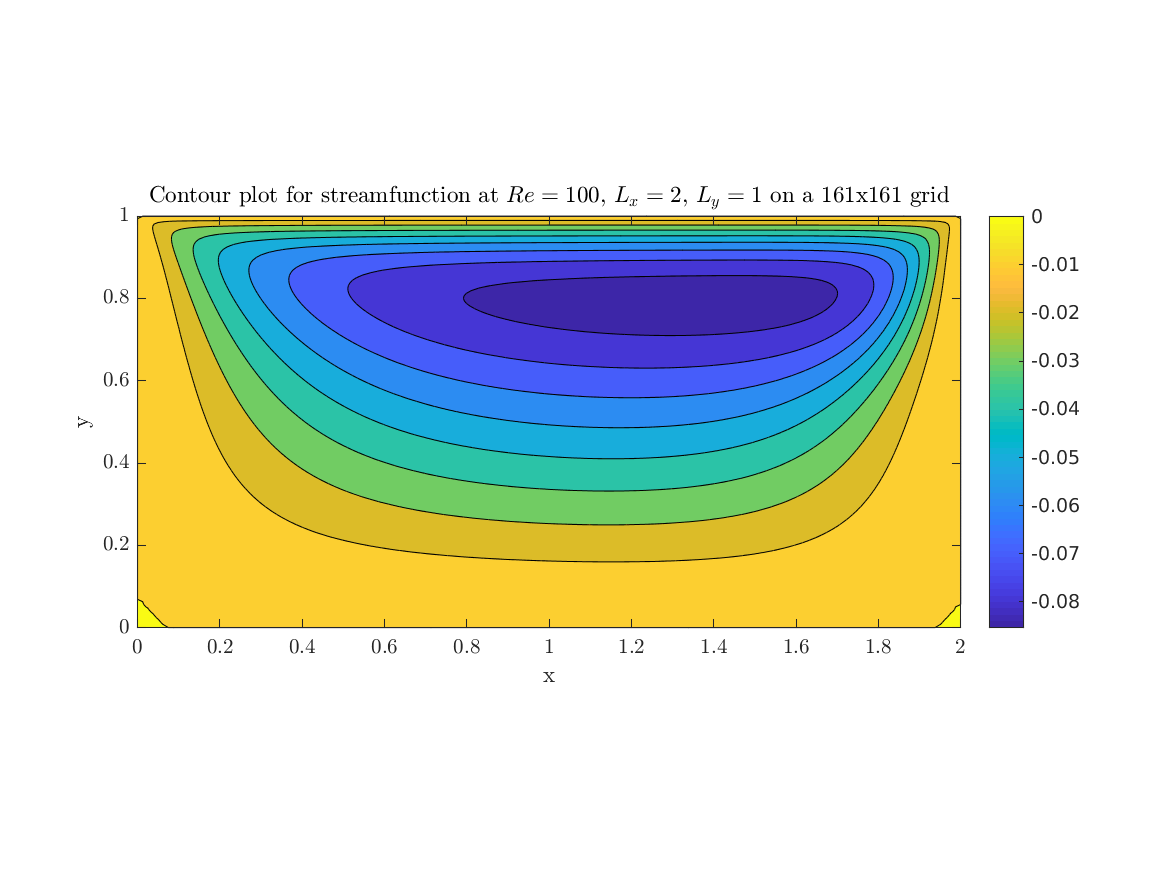
\includegraphics[width=0.60\linewidth]{../Images/lx2ly1.png}
%		\captionof{figure}{Contour plot of streamfunction at $Re=100$ on a $161 \times 161$ grid and $L_x = 2, \, L_y = 1$.}
%		\label{fig:lx2ly1}
%	\end{figure}
		
	\section{Discussion of Parallel Code}
	For the code, there are 4 main steps as outlined in the brief. For the the calculation of the vorticity boundary conditions, it was chosen not to parallelise this segment of the code as the additional time penalty required for communication outweighed the performance gain in distributing the task among processes, since only simple calculations on the edges of the matrix are required in this step.
	\vspace{0.3cm}
	\begin{wrapfigure}{r}{7cm}
		\centering
		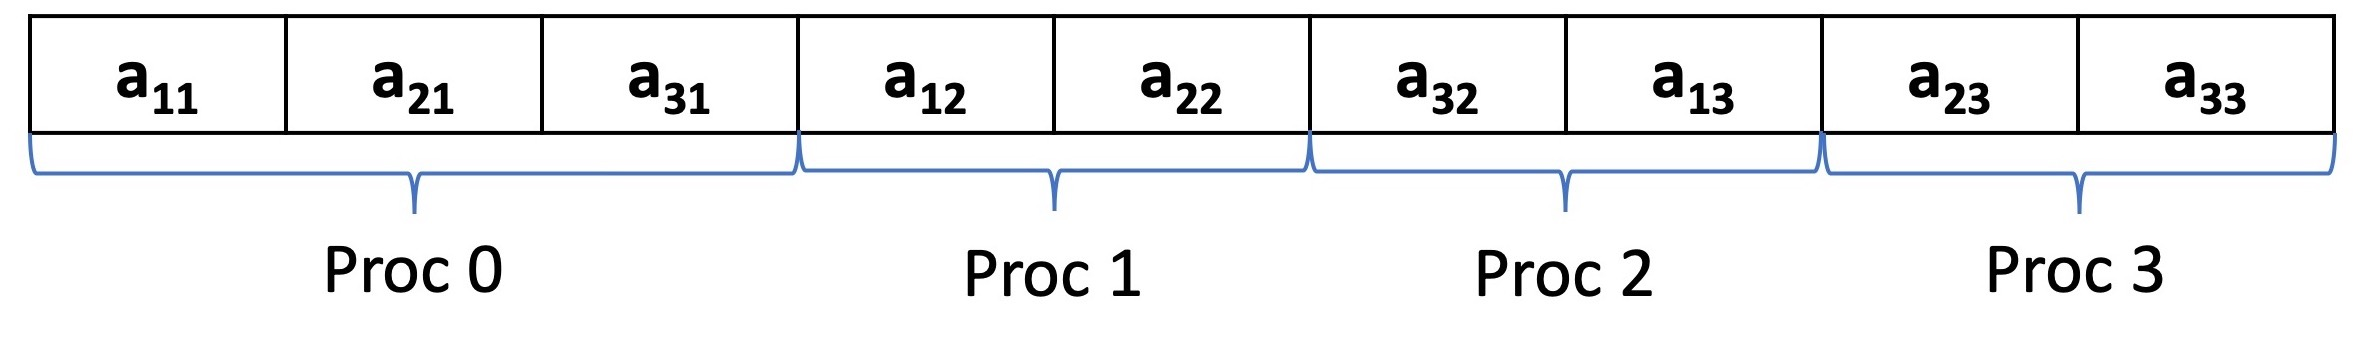
\includegraphics[width=\linewidth]{partition.jpg} 
	   	\caption{Example partitioning of column-major storage matrix among 4 processes.}
	   	\label{fig:partitioning_example}
	\end{wrapfigure}
	For the second step, the calculation of the interior vorticity at time $t$, the calculation was distributed among the processes present. The entire inner matrix was segmented out into chunks, whereby the size of each chunk is optimised such that the array is evenly distributed (no overloading of a single process). The index location of these chunks (i,j coordinates of the matrix) are then distributed to the individual processes to be solved. Since the size of the matrix remains constant throughout the solve, these coordinates only need to be calculated once. An example distribution of the process is visualised in Figure \ref{fig:partitioning_example}. The same distribution was used for the third step as well.
	
	\vspace{0.3cm}
	Additionally, the chunks are allocated in the same format as the storage format, in our case column major format. This allowed for faster memory access due to the reduced need of traversing through the array to reach the memory address. Also, as the same chunk of the array is allocated to the process each time, hence allowing for memory caching which results in faster memory access.
	
	\vspace{0.3cm}
	For the fourth step, ScaLAPACK was used to solve the system of linear equations (Ax=b). The laplacian matrix, A, was stored in a banded matrix storage format to save space. Additionally, this A matrix was prefactored via LU factorisation so as to speed up subsequent solves. The solve step was then done in parallel via ScaLAPACK.
	
	\vspace{0.3cm}
	One key decision in implementing the code was to swap around the steps of the algorithm. Since the calculation of the inner vorticity (step 2) and the boundary vorticity (step 1) are independent of one another, we can swap the steps around. By calculating the interior vorticity before the boundary, it allowed for easier parallelising of code. This is because the individual calculated segments can be summed together, as all values with index not within the range of the particular process are initialised as 0, then subsequently have the boundary condition applied. This compared to accessing the inner matrix and updating it individually, was found to be a lot more convenient and efficient. 
		
	\begin{figure}[htb]
		\centering
		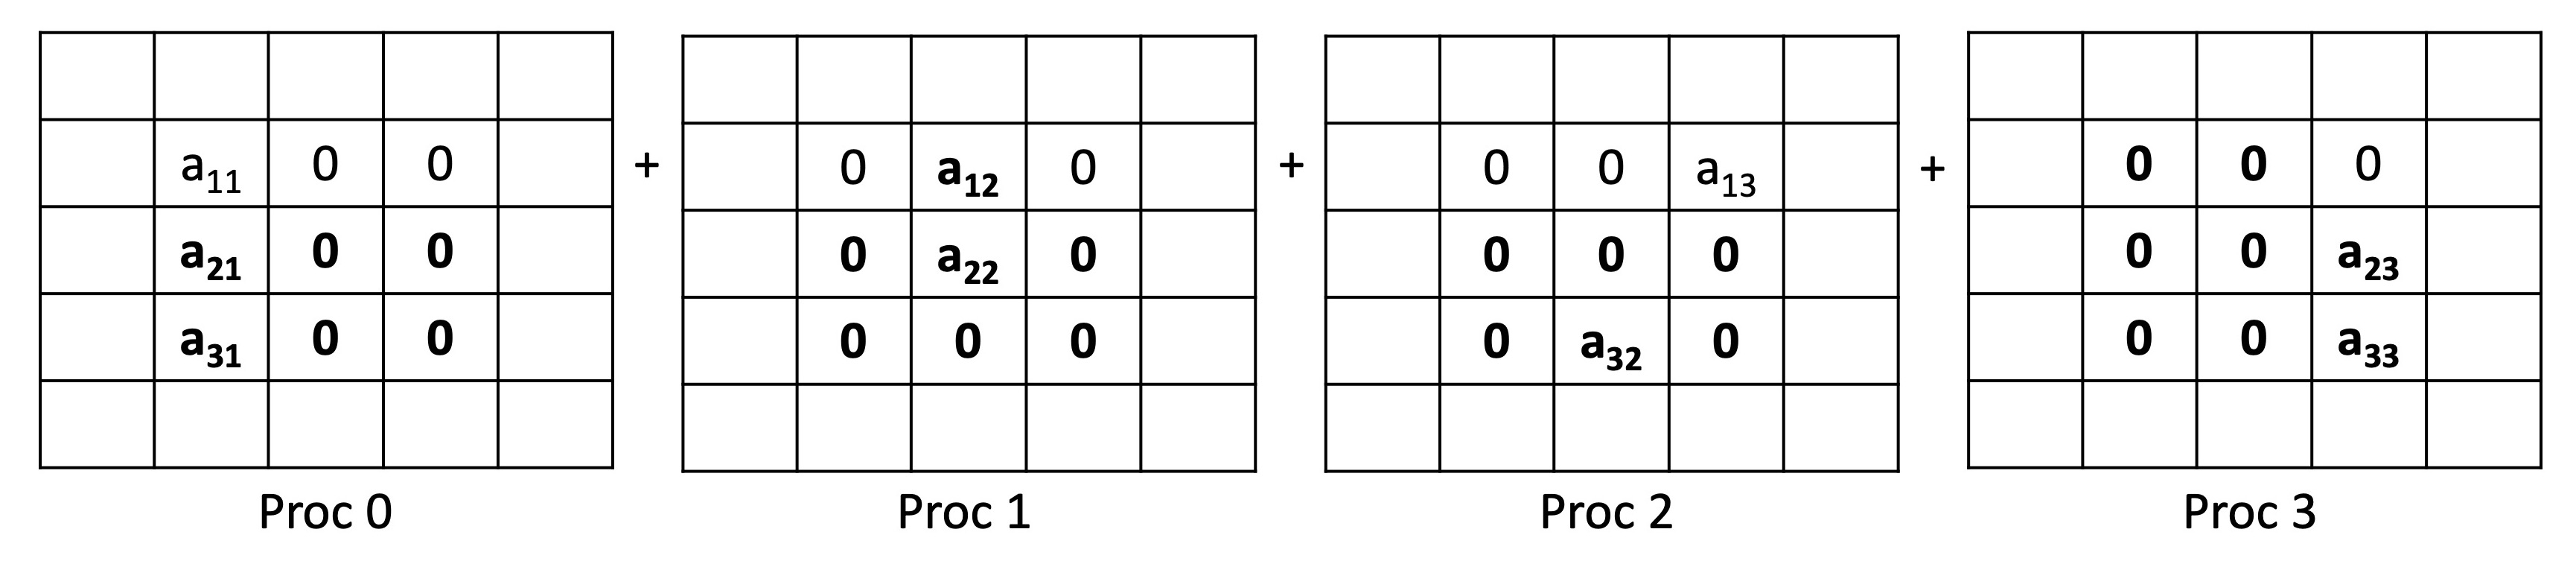
\includegraphics[width=\linewidth]{vorticity.jpg} 
	   	\caption{Example of ``overlaying" matrices to get total value}
	   	\label{fig:overlaying_example}
	\end{figure}
	
		\begin{wrapfigure}{r}{9cm}
            \centering
		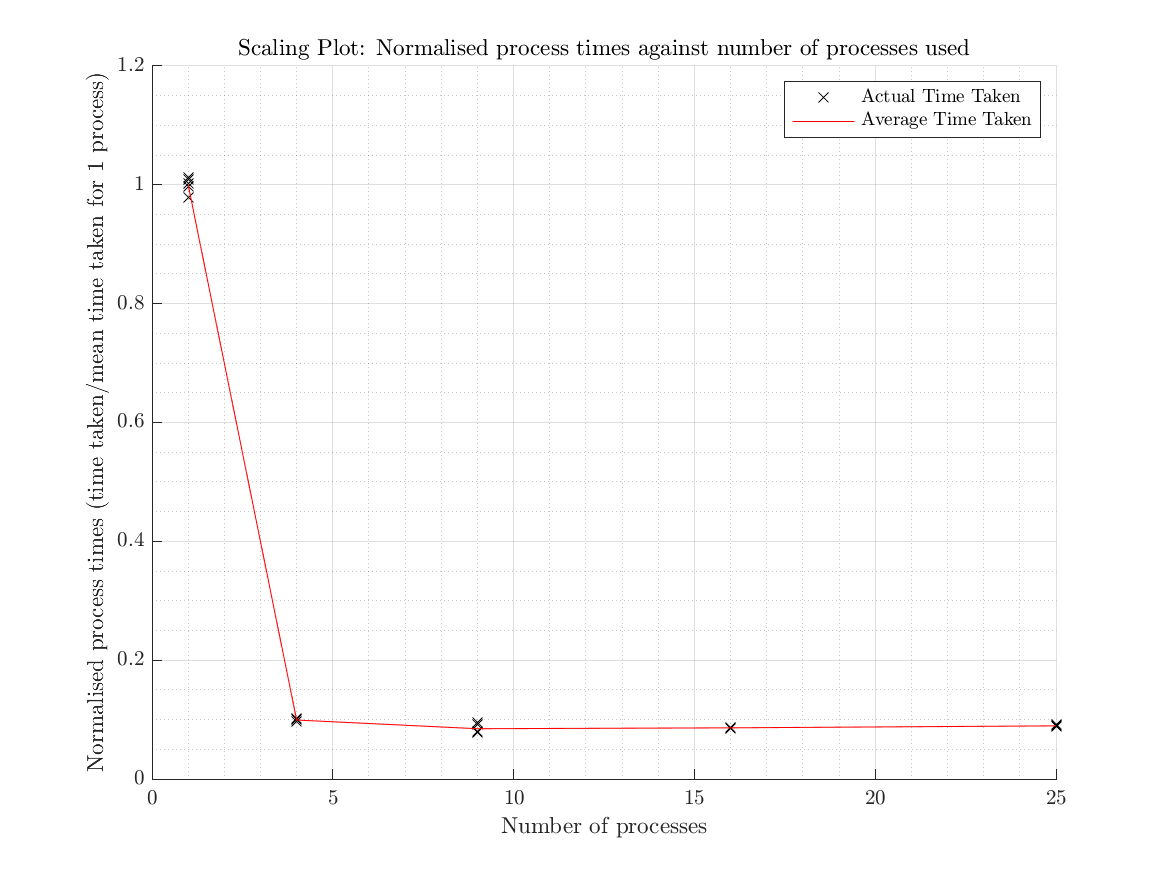
\includegraphics[width=\linewidth]{../Images/scaleplot.png} 
	   	\caption{Scale plot of time taken against number of processes}
	   	\label{fig:scaleplot}
        \end{wrapfigure}
        Another method of optimising the serial code was to separate it from the parallel one. This reduced the need for the serial code to send and receive and removed the steps of determining the local chunk of (i,j) coordinates. 
        
        \vspace{0.3cm}
        From Figure \ref{fig:scaleplot}, it is clear that parallelising the code has led to significant improvements as compared to the serial one. However, one point to note is that while moving from 4 processes to 9 processes improved the performance, beyond this, performance begins to decrease. This can be attributed to the fact that as more processes are created, more communication is required between them. In the latter case, the performance gained from splitting the work between more processes is outweighed by the performance loss due to more communication.

        
    	
%        	\begin{figure}[htb]
%        		\centering
%        		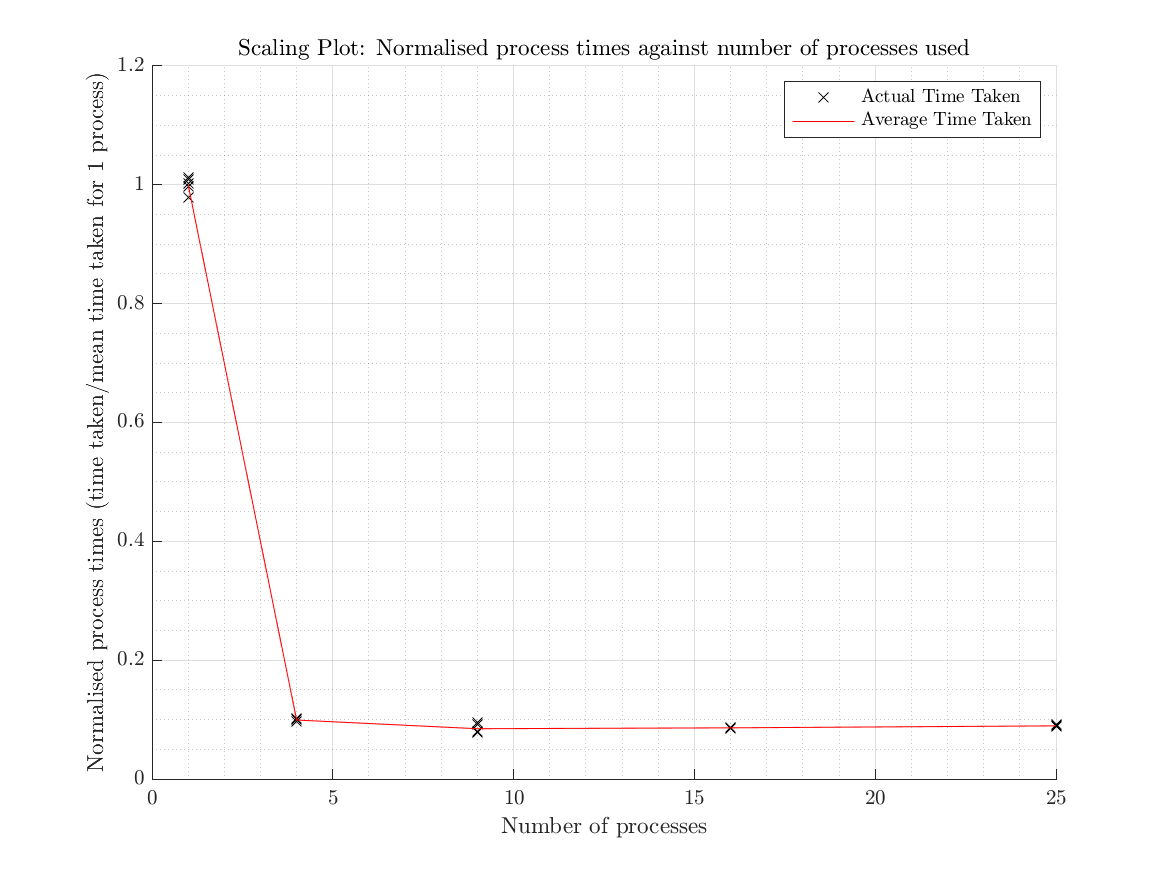
\includegraphics[width=0.5\linewidth]{../Images/scaleplot.png} 
%        	   	\caption{Scale plot of time taken against number of processes}
%        	   	\label{fig:scaleplot}
%        	\end{figure}
\end{document}